\section{Algortimi e Strutture Dati del programma}

\subsection{Strutture Dati}

Prima di descrivere gli algoritmi alla base del programma è necessario introdurre quali sono gli oggetti che verranno elaborati, come sono strutturati, anche a livello di codice, e come questi oggetti si relazionino tra di loro.

Iniziamo mostrando l'oggetto dato in ingresso all'interno del programma, ovvero la rete di automi a stati finiti. 

Brevemente, questa rete è composta da un numero di automi a stati finiti, questi automi sono collegati tra loro tramite link e all'interno degli automi questi sono composti da stati, interconnessi tramite transizioni i quali possono avere degli eventi in ingresso richiesti per l'attivazione oppure degli eventi in uscita, o entrambi. \newline

Quindi abbiamo iniziato partendo con la definizione degli elementi che risiedono alla base degli automi: gli stati, le transizioni e gli eventi. Questi oggetti sono in genere utilizzati per definire un automa a stati finiti in modo completo e dettagliato e potrebbero essere usati più o meno come struttura dati anche in altri contesti in cui non vi è necessariamente bisogno di interagire con rete di automi. \newline

Lo \textbf{stato} (\texttt{State}) è l'oggetto più semplice, rappresenta un singolo stato di un automa e ha due sole proprietà:
\begin{itemize}
    \item \textbf{id} : stringa che va a identificare univocamente l'oggetto. Potrebbe essere riferito anche come \texttt{alias} all'interno del codice
    \item \textbf{isFinal} : variabile booleana che indica se l'oggetto rappresenta uno stato finale
\end{itemize}

La \textbf{transizione} (\texttt{Transition}) invece è un collegamento orientato tra due stati e può avere o meno eventi in ingresso/uscita e/o etichette. È composta da: 
\begin{itemize}
    \item \textbf{id} : stringa che va a identificare univocamente l'oggetto. Riferito anche come \texttt{alias} all'interno del codice
    \item \textbf{start\_state} : stato iniziale da cui parte la transizione
    \item \textbf{finish\_state} : stato di arrivo della transizione
    \item \textbf{label\_oss} : stringa che indica una eventuale etichetta di osservabilità
    \item \textbf{label\_rel} : stringa che indica una eventuale etichetta di rilevanza
    \item \textbf{input\_event\_func} : un oggetto \texttt{EventFunction} che indica un possibile evento necessario in ingresso per l'attivazione della transizione
    \item \textbf{output\_events\_func} : un oggetto \texttt{EventFunction} che indica un possibile evento in uscita generato dall'attivazione della transizione
\end{itemize}
Nel caso di default, in cui non ci sono etichette di osservabilità e di rilevanza, tali etichette vengono istanziate come \(\epsilon\) mentre nel caso in cui non ci siano eventi in ingresso o in uscita questi vengono settati come \texttt{None}. \newline

Gli oggetti \texttt{EventFunction} verranno descritti a breve. Prima è necessario introdurre l'oggetto \textbf{evento} (\texttt{Event}) che rappresenta un generico evento. L'unica proprietà contenuta in evento è:
\begin{itemize}
    \item \textbf{id} : stringa che va a identificare univocamente l'oggetto. Riferito anche come \texttt{alias} all'interno del codice
\end{itemize}

Con questi tre oggetti è quindi possibile rappresentare un'\textbf{automa a stati finiti}, in inglese Finite-State Automata o in breve \texttt{FA}, come verrà principalmente chiamato da qui in avanti. È formato da:
\begin{itemize}
    \item \textbf{id} : stringa che va a identificare univocamente l'oggetto. Riferito anche come \texttt{alias} all'interno del codice
    \item \textbf{list\_states} : una lista contenente gli stati che appartengono al \texttt{FA}
    \item \textbf{list\_trans} : una lista contenente le transizioni tra stati che appartengono al \texttt{FA}
    \item \textbf{initial\_state} : lo stato iniziale del \texttt{FA}
    \item \textbf{actual\_state} : uno stato che identifica lo stato attuale durante l'esecuzione dell'automa\footnote{Questo attributo non è indispensabile per il compito del programma in senso stretto ma può essere utile in futuro qualora ampliando il programma si necessiti dell'esecuzione dell'automa.}
\end{itemize}
In questo modo si descrive un \texttt{FA} come l'insieme dei suoi stati, delle sue transizioni e dello stato iniziale. 
Nel momento in cui si hanno più \texttt{FA} che sono interconnessi tra loro si andrà a introdurre il \textbf{link} il quale descrive un collegamento tra due automi con un possibile evento caratterizzante. Un oggetto \texttt{link} è quindi composto da:
\begin{itemize}
    \item \textbf{id} : stringa che va a identificare univocamente l'oggetto. Riferito anche come \texttt{alias} all'interno del codice
    \item \textbf{start\_FA} : \texttt{FA} iniziale da cui parte il link
    \item \textbf{finish\_FA} : \texttt{FA} finale dove termina il link
    \item \textbf{contenuto} : attributo che andrà a contenere un \texttt{Evento} che va a caratterizzare il link. Riferito anche come \texttt{buffer} all'interno del codice
\end{itemize}
Come promesso, andiamo a descrivere l'oggetto \texttt{EventFunction}. Questo oggetto ha il compito di racchiudere un link e un evento associato. Come oggetto di per sé è ridondante ma ha permesso di garantire la correttezza del programma semplificando non poco la realizzazione del codice in quanto permette di rendere più leggere alcune fasi di controllo all'interno degli algoritmi. 
Come anticipato, è composto da:
\begin{itemize}
    \item \textbf{event} : l'evento che caratterizza il link tra i due automi
    \item \textbf{link} : il collegamento tra i due automi
\end{itemize}
A tutti gli effetti \texttt{EventFunction} è un oggetto di supporto all'interno del programma.

Infine, per descrivere la \textbf{rete} di automi semplicemente si racchiudono gli \texttt{FA} e i \texttt{link} nell'oggetto \texttt{Net}:
\begin{itemize}
    \item \textbf{list\_FA} : lista contenente i \texttt{FA} che appartengono alla rete
    \item \textbf{list\_link} : lista contenente i collegamenti tra i vari \texttt{FA} della rete
\end{itemize}

Questi sono le strutture dati utilizzate all'interno del programma per manipolare le reti di automi e tramite queste classi è possibile applicare degli algoritmi per generare nuove strutture. \newline

Ciò che ora è possibile generare tramite gli oggetti qui sopra presentati con il programma sono gli \textbf{spazi comportamentali}, il \textbf{diagnosticatore} e gli \textbf{spazi delle chiusure}. 
Tali oggetti saranno fondamentali per eseguire analisi sul comportamento della rete di automi ed effettuare diagnostiche. Andiamo ora a descrivere le loro strutture dati. \newline

Così come si è partiti con gli stati per descrivere le \texttt{FA} inizieremo a descrivere gli spazi comportamentali dai \textbf{nodi} (\texttt{Node}). Tali nodi descrivono un possibile stato della rete di automi. È formato da:
\begin{itemize}
    \item \textbf{id} : stringa che identifica univocamente il nodo
    \item \textbf{alias} : stringa che descrive brevemente il valore degli stati e dei link in quel nodo. Utile per stampare a video il valore del nodo in maniera leggibile
    \item \textbf{final} : variabile booleana che  indica se il nodo è un nodo finale
    \item \textbf{list\_states\_FA} : vettore contenente gli stati che appartengono a tale nodo, ogni stato è riferito a un diverso \texttt{FA}
    \item \textbf{list\_values\_link} : vettore contenente i valori attuali dei link in base agli eventi azionati
    \item \textbf{index\_oss} : numero che identifica l'indice di osservazione del nodo. Usato per creare spazi comportamentali relativo a un'osservazione
\end{itemize}
Per indicare un collegamento tra due nodi useremo una \textbf{rotta} \texttt{Route}, paragonabile a una transizione per gli automi. È caratterizzato da:
\begin{itemize}
    \item \textbf{id} : stringa che va a identificare univocamente l'oggetto. Riferito anche come \texttt{alias} all'interno del codice 
    \item \textbf{start\_node} : nodo iniziale da cui parte la rotta
    \item \textbf{finish\_node} : nodo di arrivo della rotta
    \item \textbf{label\_oss} : stringa che indica una eventuale etichetta di osservabilità
    \item \textbf{label\_rel} : stringa che indica una eventuale etichetta di rilevanza
    \item \textbf{set\_label\_rel} :  un insieme contenente etichette di rilevanza. Necessario per l'algoritmo \texttt{EspressioniRegolari}
    \item \textbf{rif\_node} : nodo di riferimento usato per l'algoritmo \texttt{EspressioniRegolari}
\end{itemize}
I due campi label sono di ridondanza ma semplificano il codice evitando di accedere necessariamente alla transizione/link di riferimento mantenendo comunque la correttezza del programma.
Gli ultimi due attributi sono utili per la risoluzione delle espressioni regolari con le etichette di rilevanza per mezzo dell'algoritmo \texttt{EspressioniRegolari} in quanto permettono di gestire le stringhe in riferimento al rispettivo nodo finale (\texttt{rif\_node}) e di gestire facilmente le operazioni di concatenazione tra stringhe adoperando \texttt{set\_label\_rel}. \newline

Le rotte e i nodi sono quindi gli oggetti fondamentali per generare gli \textbf{spazi comportamentali} (\texttt{Behavior\_Space}), semplicemente formati da:
\begin{itemize}
    \item \textbf{initial\_node} : nodo iniziale dello spazio comportamentale. Generalmente composto dagli stati iniziali degli \texttt{FA} 
    \item \textbf{list\_nodes} : lista contenente i nodi appartenenti allo spazio comportamentale
    \item \textbf{list\_routes} : lista contenente i collegamenti tra i vari nodi dello spazio comportamentale
\end{itemize}

Descrivono in modo sintetico lo spazio comportamentale e la loro struttura permette di essere sfruttati sia nel caso generale in cui lo spazio è l'insieme di tutti i comportamenti possibili dalla rete di \texttt{FA} sia nel caso relativo a una osservazione particolare data.

L'altro spazio che è possibile generare dal programma è il cosiddetto \textbf{spazio delle chiusure}. Iniziamo descrivendo cosa le \textbf{chiusure} sono.

Innanzitutto un \textbf{nodo chiusura} (\texttt{Closure\_Node}) altro non è che un nodo adoperato nelle chiusure. È semplicemente formato da:
\begin{itemize}
    \item \textbf{node} : un oggetto nodo che comporrà la chiusura
    \item \textbf{label} : una etichetta assegnata al nodo della chiusura qualora prevista
\end{itemize}
I \texttt{Closure\_Nodes} aiutano a differenziare i nodi usati negli spazi comportamentali da quelli appartenenti alle chiusure con l'aggiunta di poter contenere una etichetta al loro interno, utile per la successiva diagnosi. 

Vari nodi chiusura permettono di comporre una \textbf{chiusura} (\texttt{Closure}), composta da:
\begin{itemize}
    \item \textbf{id} : stringa che identifica univocamente la chiusura
    \item \textbf{initial\_node} : nodo iniziale della chiusura. Generalmente è univoco all'interno di uno spazio delle chiusure
    \item \textbf{list\_nodes} : lista contenente i nodi appartenenti alla chiusura
    \item \textbf{list\_routes} : lista contenente i collegamenti tra i vari nodi della chiusura
    \item \textbf{delta} : stringa contenente il \texttt{delta} della chiusura
    \item \textbf{list\_diagnostic\_output\_route} : lista contenente le rotte in uscita dalla chisura verso nodi esterni alla chiusura stessa
\end{itemize}
La struttura di una chiusura è simile a quella di uno spazio comportamentale sebbene i loro scopi siano differenti.

L'insieme di più chisure (univoche rispetto al nodo iniziale) può andare a formare lo \textbf{spazio delle chiusure} (\texttt{Closure\_Space}), necessario per il successivo lavoro di diagnostica. È formato banalmente da:
\begin{itemize}
    \item \textbf{list\_closures} : lista delle chiusure appartenenti allo spazio
    \item \textbf{list\_routes} : lista contenente i collegamenti tra le varie chiusure dello spazio
\end{itemize}

L'ultimo oggetto da descrivere è il \textbf{diagnosticatore}. Questo altro non è che un riassunto dello spazio delle chiusure dove ogni chiusura viene semplificata come uno stato contenente il minimo quantitativo di informazione necessaria per la diagnosi. Pertanto introduciamo lo \textbf{stato diagnostico} (\texttt{State\_Diagnostic}) contenente:
\begin{itemize}
    \item \textbf{id} : stringa identificativa dello stato. Eredita l'id della chiusura relativa
    \item \textbf{alias} : stringa contenente il nome dello stato. Principalmente utile per stampare a video in modo leggibile il diagnosticatore
    \item \textbf{delta} : \texttt{delta} della chiusura qualora ne sia provvisto
    \item \textbf{list\_routes} : lista delle rotte uscenti dalla chiusura
\end{itemize}

Le rotte adoperano la classe \textbf{Route\_Diagnostic}, ereditata da \texttt{Route} usata per il contesto del diagnosticatore. Risiedono all'interno degli stati in quanto una singola rotta dello spazio comportamentale potrebbe ripresentarsi più volte nello spazio delle chiusure. In questo ogni stato ha tutti i riferimenti chiave della rispettiva chiusura.

Il \textbf{diagnosticatore} (\texttt{Diagnosticator\_Space}) è infine formato da:
\begin{itemize}
    \item \textbf{list\_states} : lista contenente gli stati del diagnosticatore
    \item \textbf{initial\_state} : stato iniziale del diagnosticatore
\end{itemize}
Tramite il \texttt{Diagnosticatore} è quindi possibile eseguire la diagnosi attraverso gli algoritmi che verranno mostrati e descritti nel prossimo paragrafo.
\subsection{Algoritmi}
Come già accennato, il nostro programma si occupa, data in input la definizione di una rete, di calcolare il relativo spazio comportamentale, quello relativo a un'osservazione lineare (che chiameremo spazio osservabile), la diagnosi relativa a quest'ultimo, la chiusura silenziosa e lo spazio delle chiusure, oltre al diagnosticatore e alla diagnosi lineare relativa a una osservazione lineare data.
In sintesi:
\begin{itemize}
    \item Generazione spazio comportamentale
    \item Generazione spazio comportamentale da osservazione lineare (spazio osservabile)
    \item Diagnosi relativa a una osservazione lineare
    \item Generazione spazio delle chiusure silenzione (e decorazione)
    \item Generazione diagnosticatore
    \item Diagnosi lineare relativa a una osservazione lineare
\end{itemize}

All'interno del GitHub del progetto è possibile accedere a tutti i pseudocodici e alle varie funzioni del programma scritto in python citate nelle seguenti sezioni.
\subsubsection{Generazione spazio comportamentale}
Il primo step dell’algoritmo consisteva nel creare lo spazio compartimentale partendo dalla definizione di una rete di automi. 
Lo pseudo codice è illustrato di seguito.

\begin{algorithm}[H]
\SetAlgoLined
\KwResult{BEHAVIOR\_SPACE}
 \textit{new} list\_space\_nodes as empty list\;
 \textit{new} list\_routes as empty list\;
 \textit{new} tail\_nodes as empty list\;
 \;
 \textit{new} initial\_node as (Net.get\_state\_list\_FAs, Net.get\_content\_list\_LINKs)\;
 \textit{set} initial\_node.final as True\;
 \;
 \textit{add} initial\_node to list\_space\_nodes\;
 \textit{add} initial\_node to tail\_nodes\;
 \While{tail\_nodes is not empty}{
  \textit{get} tail\_nodes.firstElement as node\_current\;
  \ForAll{state\_FA in node\_current.state\_list\_FAs}{
    \ForAll{transaction in state\_FA.output\_transaction}{
        \If{transaction.event couples is present in node\_current.content\_list\_LINKs}{
            \textit{get} transaction.finish\_state as new\_state\;
			\textit{get} transaction.output\_events as link\_events\_to\_update\;
			\;		
			\textit{new} node\_to\_add as copy of node\_current\;
			\textit{update} state\_FA in node.state\_list\_FAs with new\_state\;
			\textit{update} content\_list\_LINKs couples with link\_events\_to\_update\;
			\;
			\textit{new} route\_to\_add as (node\_current, transaction, node\_to\_add)\;
			\textit{add} route\_to\_add to list\_routes\;
			\If{node\_to\_add is not in list\_space\_nodes}{
			    \If{all node\_to\_add.content\_list\_LINKs has empty link.content}{
			        \textit{set} node\_to\_add.final as True\;
			    }
			    \textit{add} node\_to\_add to list\_space\_nodes
				tail\_nodes.push(node\_to\_add)
			}
		}
    }
    
  }
  tailNodi.pop()
 }
 \caption{Generazione Spazio Comportamentale}
 \rememberlines
\end{algorithm}

\begin{algorithm}[H]
\resumenumbering
\SetAlgoLined
\KwResult{BEHAVIOR\_SPACE}
 \# PRUNING\;
 BFS(foreach list\_space\_nodes where node.final is True, list\_routes)\;
 \ForAll{node in list\_space\_nodes}{
    \textit{set} node.alias as incremental(id) 
 }
 \textit{new} BEHAVIOR\_SPACE as (initial\_node, list\_space\_nodes, list\_routes)
 \caption{Generazione Spazio Comportamentale}
\end{algorithm}
Nel nostro programma, il corrispettivo risulta essere la funzione \textbf{generate\_behavior\_space}.
Inizialmente si creava il nodo iniziale contenente gli stati iniziali delle FA e il contenuto iniziale dei link (tutti vuoti).
Successivamente si cicla su una coda, costituita inizialmente dal nodo iniziale:
\begin{enumerate}
    \item Si prende il primo elemento del nodo e si controllano tutti gli stati attuali.
    \item Per ogni stato analizzato si itera sulle transazioni in uscita e se l’evento della transazione è attivabile (dunque tale evento in ingresso è attualmente presente nel corrispettivo link del nodo analizzato) si crea il nuovo nodo che differenzia da quello analizzato in base alla transazione attivata: \begin{itemize}
        \item avrà uno stato diverso nella lista degli stati in base allo stato di arrivo della transazione
        \item avrà dei contenuti dei link diversi in base agli eventi in uscita della transazione
    \end{itemize}
    \item Nel codice, il compito di questo passaggio è affidato alla funzione in \textit{extrafunction}, denominata \textbf{change\_state}.
    \item Se il nodo non è presente nello spazio lo si aggiunge alla spazio e alla coda dei nodi
    \item Si aggiunge una nuova transizione  tra il nodo appena creato e quello di partenza
    \item Se il nodo presenta il contenuti dei suoi link vuoti lo si imposta come nodo finale di accettazione
    \item Si rimuove il nodo analizzato
\end{enumerate}
In seguito si esegue una potatura di tutti quei nodi che non portano a un nodo iniziale (con le rispettive transizioni) attraverso un algoritmo di \textbf{BFS} (nel nostro programma utilizziamo la funzione omonima presente nel file \textit{extrafunction}, scritta da noi), che per ogni nodo finale dato, restituisce tutti i nodi che portano a quel nodo, alla fine della analizzi avremo dei nodi che non sono mai stati “utilizzati”, dunque che sarà necessario rimuovere, perché potrebbero generare dei cicli o punti morti.

BFS altro non è l'algoritmo \textbf{Breadth-First Search} leggermente modificato per essere applicato al nostro caso, dove il grafo è il nostro spazio comportamentale, la direzione degli archi è invertita e il nodo iniziale è uno dei nodi finali. Se qualche nodo non viene toccato dopo l'esecuzione dell'algoritmo vuol dire che quel nodo non raggiunge il nodo finale e quindi verrà potato qualora non raggiunga nessun nodo finale presenti nello spazio comportamentale.

Infine, si rinomina i nodi rimanenti con un id crescente
\subsubsection{Generazione Spazio Osservabile}
Il secondo passaggio richiesto è quello di generare uno spazio comportamentale osservabile, partendo dalla definizione della rete e una lista di osservazioni, cioè una lista di etichette di osservabilità.

\begin{algorithm}[H]
\SetAlgoLined
\KwResult{OSSERVABLE\_SPACE}
 \textit{new} list\_space\_nodes as empty list\;
 \textit{new} list\_routes as empty list\;
 \textit{new} tail\_nodes as empty list\;
 \;
 \textit{new} initial\_node as (Net.get\_state\_list\_FAs, Net.get\_content\_list\_LINKs)\;
 \textit{set} initial\_node.final as True\;
 \textit{add} initial\_node to list\_space\_nodes\;
 \textit{add} initial\_node to tail\_nodes\;
 \While{tail\_nodes is not empty}{
  \textit{get} tail\_nodes.firstElement as node\_current\;
  \ForAll{state\_FA in node\_current.state\_list\_FAs}{
    \ForAll{transaction in state\_FA.output\_transaction}{
        \If{transaction.event couples is present in node\_current.content\_list\_LINKs, index\_oss = 0}{
            \If{transaction.osservation\_label exist and transaction.osservation\_label is not the next(list\_osservable) from node.index\_oss}{
                \textbf{break}\;
            }
            \textit{get} transaction.finish\_state as new\_state\;
			\textit{get} transaction.output\_events as link\_events\_to\_update\;
			\textit{new} node\_to\_add as copy of node\_current\;
			\textit{update} state\_FA in node.state\_list\_FAs with new\_state\;
			\textit{update} content\_list\_LINKs couples with link\_events\_to\_update\;
			\textit{new} route\_to\_add as (node\_current, transaction, node\_to\_add)\;
			\textit{add} route\_to\_add to list\_routes\;
			\If{node\_to\_add is not in list\_space\_nodes}{
			    \If{all node\_to\_add.content\_list\_LINKs has empty link.content and index\_oss is equal len(list\_osservable)}{
			        \textit{set} node\_to\_add.final as True\;
			    }
			    \textit{add} node\_to\_add to list\_space\_nodes
				tail\_nodes.push(node\_to\_add)
			}
		}
    }
    
  }
  tailNodi.pop()
 }
 \caption{Generazione Spazio Comportamentale}
 \rememberlines
\end{algorithm}

\begin{algorithm}[H]
\SetAlgoLined
\resumenumbering
\KwResult{OSSERVABLE\_SPACE}
 \# PRUNING\;
 BFS(foreach list\_space\_nodes where node.final is True, list\_routes)\;
 \ForAll{node in list\_space\_nodes}{
    \textit{set} node.alias as incremental(id) 
 }
 \textit{new} OSSERVABLE\_SPACE as (initial\_node, list\_space\_nodes, list\_routes)
 \caption{Generazione Spazio Comportamentale}
\end{algorithm}
Rispetto all'algoritmo precedente, quello di generazione dello spazio comportamentale, si aggiungono unicamente due condizioni in più:

\begin{itemize}
    \item \textbf{STEP 2} $\rightarrow $ Per ogni stato analizzato si itera sulle transazioni in uscita e se l’evento della transazione è attivabile (dunque tale evento in ingresso è attualmente presente nel corrispettivo link del nodo analizzato) e \textbf{se la sua etichetta di osservabilità è nulla oppure è il successivo elemento della lista di osservabilità}, si crea il nuovo nodo che differenzia da quello analizzato in base alla transazione attivata:
    \begin{itemize}
        \item $\dots$
        \item \textbf{avrà come indice di osservazione incrementato di uno rispetto al nodo analizzato.}
    \item \textbf{STEP 6} $\rightarrow $ Se il nodo presenta il contenuto dei suoi link come vuoti e l\textbf{’indice di osservazione pari alla lunghezza della lista di osservabilità}, lo si imposta come nodo finale di accettazione
    \end{itemize}
\end{itemize}
Segue BFS e generazione indici.

Riassumendo, vengono aggiunti i nodi in modo da creare percorsi che portano a dei nodi finali nei quali sono presenti transazioni contenenti o etichette di osservabilità nulle oppure, se presenti, coerenti con l’ordine dato dalla lista di osservabilità
\subsubsection{Diagnosi relativa a osservazione lineare}
La terza fase consiste nel produrre la diagnosi dello spazio osservabile, che risulterà essere un'espressione regolare.
Lo pseudo codice è illustrato di seguito.

\begin{algorithm}[H]
\SetAlgoLined
\KwResult{listRoutes-Diagnosis}
 new listRoutes as copy of OssSpace.listRoutes\;
 new listNodes as coppy of OssSpace.listNodes\;
 new initial\_node as copy of OssSpace.initial\_node\;
 \;
 \If{initial\_node is present in route in listRoutes as finish\_node}{
    new new\_initial\_node\;
	set new\_initial\_node.isFinal as True\;
	\;	
	new new\_route as <new\_initial\_node, 'empty', initial\_node>\;
	\;	
	add new\_initial\_node to listNodes\;
	add new\_route to listRoutes\;
	\;	
	update initial\_node with new\_initial\_node\;
 }
 new final\_node\;
 set final\_node.isFinal as True\;
 \;
 new count\_acept as count(node in  listNodes where isFinal is True)\;
 \If{count\_acept $>$ 1 or (count\_acept is 1 and exist route in listRoutes as start\_node is node in listNodes where isFinal is True and start\_node is not finish\_node}{
    \ForAll{node in  listNodes where isFinal is True}{
        new new\_route as <node, 'empty', final\_node>\;
		add new\_route to listRoutes\;
    }
 }
 \caption{Diagnosi relativa a osservazione lineare}
 \rememberlines
\end{algorithm}

\begin{algorithm}[H]
\resumenumbering
\SetAlgoLined
\KwResult{listRoutes-Diagnosis}
 \While{listRoutes has more than 1 element}{
     \uIf{exist sequence $[<n,r\_1, n\_1>, <n\_1,r\_2,n\_2>,...,<n\_(k-1), r\_k, n'>]$ of routes in listRoutes where all node n\_i have only the sequence routes }{
        remove sequence routes in listRoutes\;
    	add new\_route as $<n, concat(r\_i), n')>$ to listRoutes\;
    }
    \uElseIf{exist routes with same n as start\_node and n' as finish\_node} {
        remove sequence routes in listRoutes\;
		add new\_route as $<n, concat(routes, '|'), n')>$ to listRoutes\;
    }
    \Else{
        take n from listNodes with n is not initial\_node and n is not the final\_node\;
        \ForAll{routes as $<n', r', n>$ where finish\_node is n}{
            \ForAll{routes as $<n, r'', n'>$ where start\_node is n}{
                \eIf{exist route as $<n,r,n>$ where star\_node and finish\_node are n}{
                    add new\_route as $<n', r'(r*)r'', n''>$ to listRoutes\;
                }
                {
                    add new\_route as $<n', r'r'', n''>$ to listRoutes\;
                }
            }
        }
        remove n from listNodes\;
        remove routes from listRoutes where n is start\_node or finish\_node\;
    }
 }
 \caption{Diagnosi relativa a osservazione lineare}
\end{algorithm}

La funzione responsabile di questo passaggio è quella presente nel file \textit{extrafunction} con il nome \textbf{reg\_expr}, la quale implementazione varia leggermente rispetto all’algoritmo proposto.

Per produrre in uscita una espressione regolare è necessario seguire questi steps:
\begin{enumerate}
    \item Se il nodo iniziale ha transizioni in entrata, allora bisogna creare un nuovo nodo iniziale temporaneo che avrà solamente una transizione vuota in uscita verso il vecchio nodo iniziale
    \item Si crea un nodo finale e tutti i nodi di accettazione presenti nello spazio verranno connessi a questo mediante una transizione vuota in uscita.
    \item Poi, finchè sono presenti dei nodi che non sono quello iniziale e finale si eseguiranno questi step:
    \begin{enumerate}
        \item Si prende un nodo random tra quelli attualmenti presenti
        \item Se presenta più transizioni in uscita verso gli stessi nodi, queste verranno raggruppate in un’unica transizione verso il rispettivo nodo che avrà come etichetta di rilevanza, le etichette di rilevanza delle transizioni d’origine unite tramite un \textbf{OR}
        \item Se invece presenta solo una transizione in entrata e in uscita, allora il nodo verrà rimosso e le due transazioni concatenate in \textbf{AND}
        \item Se invece le transizioni in entrata o in uscita sono molteplici, si combinano tutte le transizioni in entrata e in uscita, creando delle nuove transizioni che avranno come etichetta di rilevanza \textbf{AND} tra l’etichetta di quella in ingresso considerata e quella di uscita. Inoltre se il nodo presenta delle \textit{autotransizioni}, tra le due etichette verrà frapposto in \textbf{AND} anche l’etichetta dell’\textit{autotransizione} con il simbolo di molteplicità.
    \end{enumerate}
\end{enumerate}
In conclusione, rimarrà un’unica transizione con un’etichetta di rilevanza che risulterà essere il raggruppamento di tutte le transizioni dello spazio.
\subsubsection{Generazione dello spazio delle chiusure silenziose}

La successiva fase consiste nel generare lo spazio delle chiusure partendo dallo spazio comportamentale.
Lo pseudo codice è illustrato di seguito ed è diviso in due parti, la prima per generare la chiusura silenziosa, l'altra per generare iterativamente lo spazio delle chiusure.

\begin{algorithm}[H]
\SetAlgoLined
\KwResult{SILENCE\_CLOSING}
 new list\_closing\_nodes as empty list\;
 new list\_closing\_routes as empty list\;
 new list\_output\_routes as empty list\;
 new tail\_nodes as empty list\;
 \;
 \If{node not exist in list\_space\_nodes}{
    \textbf{ERROR}\;
 }
 \;
 new initial\_node as copy of node\;
 add initial\_node to list\_closing\_nodes\; 
 add initial\_node to tail\_nodes\;
 
 \While{tail\_nodes is not empty}{
    get tail\_nodes.firstElement as node\_current\;
    \ForAll{route in osservable\_space.list\_routes where route.start\_node is node\_current}{
        \eIf{route.label\_osservation not exist}{
            get route.finish\_node as node\_to\_add
			add ruote to list\_closing\_routes 
			\;	
			\If{node\_to\_add is not in list\_closing\_nodes}{
			    add node\_to\_add to list\_closing\_nodes
				tail\_nodes.push(node\_to\_add)
			}
        }
        {
            add route to list\_output\_routes
        }
    }
    pop tail\_node\;
 }
 
 \caption{Generazione spazio delle chiusure}
\end{algorithm}

Le funzioni che si occupano di questo passaggio sono due, ovvero \textbf{generator\_silence\_closure} che viene chiamata iterativamente da \textbf{generator\_closures\_space}.
Per creare una chiusura silenziosa è necessario specificare un nodo di partenza e lo spazio comportamentale
\begin{enumerate}
    \item Si crea il nodo iniziale della chiusura che corrisponderà a quello di partenza dato.
    \item Lo si aggiunge a una coda
    \item Finchè la coda ha elementi, si prende il primo elemento e lo si analizza
    \item Per ogni transizione nello spazio comportamentale che ha quel nodo come nodo di partenza, se l’etichetta di osservabilità è nulla, allora si crea un nuovo nodo per la chiusura silenziosa
    \item lo si aggiunge alla coda
    \item si aggiunge la transizione alla lista delle transazioni della chiusura
    \item Se invece l’etichetta di osservabilità non è nulla, allora non si aggiunge nessun nodo ma si aggiunge la transizione alla lista delle transizioni in uscita dalla chiusura stessa (che sarà diretta a un’altra chiusura)

\end{enumerate}

\begin{algorithm}[H]
\SetAlgoLined
\KwResult{List Closing}
 new list\_closing as empty list\;
 new tail\_closing as empty list\;
 \;
 new initialize\_closing as SILENCE\_CLOSING(osservable\_space, osservable\_space.initialize\_node)\;
 add initialize\_closing to list\_closing\;
 push  to tail\_closing\;
 
 \While{tail\_closing is not empty}{
    get tail\_closing.firstElement as closing\_current\;
    \ForAll{ output\_route in closing\_current.list\_output\_routes}{
        \If{output\_route.finish\_node is not in list\_closing as closing.initialize\_node}{
            new closing\_temp as SILENCE\_CLOSING(osservable\_space, output\_route.finish\_node)\;
			\;	
			add closing\_temp to list\_closing\;
			push closing\_temp to tail\_closing\;
        }
    }
    pop tail\_closing\;
 }
 
 \caption{Generazione spazio delle chiusure}
\end{algorithm}

Nel programma corrisponde ai seguenti passi:
\begin{enumerate}
    \item Viene creata la prima chiusura silenziosa partendo dal nodo iniziale
    \item Si aggiunge la chiusura a una coda e finchè la coda ha elementi si itera:
    \begin{enumerate}
        \item Si prende la prima chiusura dalla coda e per ogni transizione in uscita si recupera il nodo di arrivo
        \item Si genera la chiusura silenziosa a partire dal nodo di arrivo e se non presente, lo si aggiunge alla coda.
        \item Si crea una transizione tra le due chiusure con gli stessi riferimenti della transizione di uscita
    \end{enumerate}
\end{enumerate}

Una volta concluso si avrà uno spazio delle chiusure silenziose.

Per ogni chiusura si trova la relativa decorazione per decorare lo spazio delle chiusure, i passaggi sono simili a quelli già visti con il calcolo della diagnosi, tranne che l’algoritmo produce in output una lista di espressioni, una per ogni stato di accettazione.

\begin{algorithm}[H]
\SetAlgoLined
\KwResult{listRoutes-Diagnosis}
 new listRoutes as copy of OssSpace.listRoutes\;
 new listNodes as coppy of OssSpace.listNodes\;
 new list\_output\_routes as copy of Closing.list\_output\_routes
 new initial\_node as copy of OssSpace.initial\_node\;
 \;
 \If{initial\_node is present in route in listRoutes as finish\_node}{
    new new\_initial\_node\;
	set new\_initial\_node.isFinal as True\;
	\;	
	new new\_route as <new\_initial\_node, 'empty', initial\_node>\;
	\;	
	add new\_initial\_node to listNodes\;
	add new\_route to listRoutes\;
	\;	
	update initial\_node with new\_initial\_node\;
 }
 new final\_node\;
 set final\_node.isFinal as True\;
 
 \ForAll{ node in listde where isFinal is True}{
    new new\_route as <node, 'empty', final\_node>
	add new\_route to listRoutes
 }
 \caption{Decorazione di una chiusura}
   \rememberlines
\end{algorithm}

E nel ciclo while

\begin{algorithm}[H]
\resumenumbering
\SetAlgoLined
\KwResult{listRoutes-Diagnosis}
\uIf{exist sequence $[<n,r\_1, n\_1>, <n\_1,r\_2,n\_2>,...,<n\_(k-1), r\_k, n'>]$ of routes in listRoutes where all node n\_i have only the sequence routes }{
        \eIf{n' is not final\_node and n\_(k-1).isFinal is False}{
            remove sequence routes in listRoutes\;
    	    add new\_route as $<n, concat(r\_i), n')>$ to listRoutes\;
    	}
    	{
    	    remove sequence routes in listRoutes\;
    	    add new\_route as $<n, concat(r\_i), n')>$ to listRoutes\;
    	    update new\_route.subscript with value n\_(k-1)\;
    	}
        
    }
    \uElseIf{exist sequence [<n,r\_1, n\_1>, <n\_1,r\_2,n\_2>,...,<n\_(k-1), r\_k.subscript is n\_p, n'>] of routes in listRoutes where all node n\_i have only the sequence routes} {
        remove sequence routes in listRoutes\;
		add new\_route as $<n, concat(r\_i), n')>$ to listRoutes
		update new\_route.subscript with value n\_p\;
    }
    \uElseIf{exist routes with same n as start\_node and n' as finish\_node}
    {
    	remove sequence routes in listRoutes\;
		add new\_route as $<n, concat(routes, '|'), n')>$ to listRoutes\;
    }
    \uElseIf{exist routes with same n as start\_node and n' as finish\_node with routes.subscript is n\_p}
    {
        move sequence routes in listRoutes\;
		add new\_route as $<n, concat(routes, '|'), n')>$ to listRoutes\;
		update new\_route.subscript with value n\_p\;
    }
    
 \caption{Decorazione di una chiusura}
 \rememberlines
\end{algorithm}

\begin{algorithm}[H]
\resumenumbering
\SetAlgoLined
\KwResult{listRoutes-Diagnosis}
\Else{
        take n from listNodes with n is not initial\_node and n is not the final\_node\;
        \ForAll{routes as $<n', r', n>$ where finish\_node is n}{
            \ForAll{routes as $<n, r'', n'>$ where start\_node is n}{
                \uIf{n'' is final\_node and (n is Final or n exist in list\_output\_routes as start\_node)}
                {
                    \eIf{exist route as $<n,r,n>$ where star\_node and finish\_node are n}{
                        add new\_route as $<n', r'(r*)r'', n''>$ to listRoutes\;
                        update new\_route.subscript with value n\;
                    }
                    {
                        add new\_route as $<n', r'r'', n''>$ to listRoutes\;
                        update new\_route.subscript with value n\;
                    }
                }
                \uElseIf{exist route as <n,r,n> where star\_node and finish\_node are n}
                {
                    add new\_route as $<n', r'(r*)r'', n''>$ to listRoutes\;
                }
                \Else{
                    add new\_route as $<n', r'r'', n''>$ to listRoutes
                }
            }
            \ForAll{all routes as <n, r'' with subscript is n\_p, n''>}{
                \eIf{exist route as <n,r,n> where star\_node and finish\_node are n}
                {
                    add new\_route as $<n', r'(r*)r'', n''>$ to listRoutes\;
					update new\_route.subscript with value n\;
                }
                {
                    add new\_route as $<n', r'r'', n''>$ to listRoutes\;
                    update new\_route.subscript with value n\;
                }
            }
        }
        remove n from listNodes\;
        remove routes from listRoutes where n is start\_node or finish\_node\;
    }
     \caption{Decorazione di una chiusura}
\end{algorithm}

La prima fase è identica a quella della diagnosi, si raggruppano tutte le transazioni dei nodi che non sono iniziali o di accettazione. 

Nella seconda fase invece si considerano i nodi di accettazione, escluso quello iniziale e quello finale e si creano tante transizioni parallele che vanno dal nodo iniziale a quello finale, quante il numero di nodi di accettazione.
Per far questo, durante la semplificazione si aggiunge anche un riferimento al nodo che è stato eliminato. Si otterrà quindi una serie di transizioni parallele.

Per ogni transizione si recupererà il nodo di riferimento e si aggiungerà una label al nodo della chiusura con il valore della etichetta di rilevanza della transizione

\subsubsection{Generazione del diagnosticatore}
Il quinto step consiste nel generare il diagnosticatore partendo dallo spazio delle chiusure. Lo pseudo codice è illustrato di seguito.

\begin{algorithm}[H]
\SetAlgoLined
\KwResult{Diagnosticator}
create list\_diagnosticated\_closing as empty list\;
\ForAll{closing in list\_closing}
{
    new delta as empty string\;
    \ForAll{node in closing.list\_closing\_nodes where node.final is True}
    {
        update delta adding node.label\;
    }
    \ForAll{output\_route in closing.list\_output\_routes}{
        update output\_route.label with start\_node.label\;
    }
    new diagnostic\_closing as $<delta, closing>$\;
    add diagnostic\_closing to list\_diagnosticated\_closing\;
}
     \caption{Generazione del diagnosicatore}
\end{algorithm}

La funzione responsabile di tale compito è \textbf{generator\_diagnosticator}. Nel nostro codice, per ottimizzare il calcolo, abbiamo creato la variante integrata nella generazione del closure space, denominata molto semplicemente \textbf{generator\_closures\_space\_and\_diagnosticator}.

Il ragionamento che sta dietro alla generazione del diagnosticatore è molto semplice, per ogni chiusura dello spazio delle chiusure decorato, si crea uno stato, che avrà come delta il valore delle label degli stati di accettazione. Ogni transizione in uscita diverrà anche una transizione tra i vari stati, ma che avrà come etichetta l’unione tra la sua etichetta e quella del nodo di partenza della chiusura (se presente).

\subsubsection{Generazione diagnosi lineare}
L’ultima fase dell’algoritmo consiste nel generare la diagnosi lineare partendo dal diagnosticatore e da un’osservazione lineare.

Lo pseudo codice è mostrato di seguito.

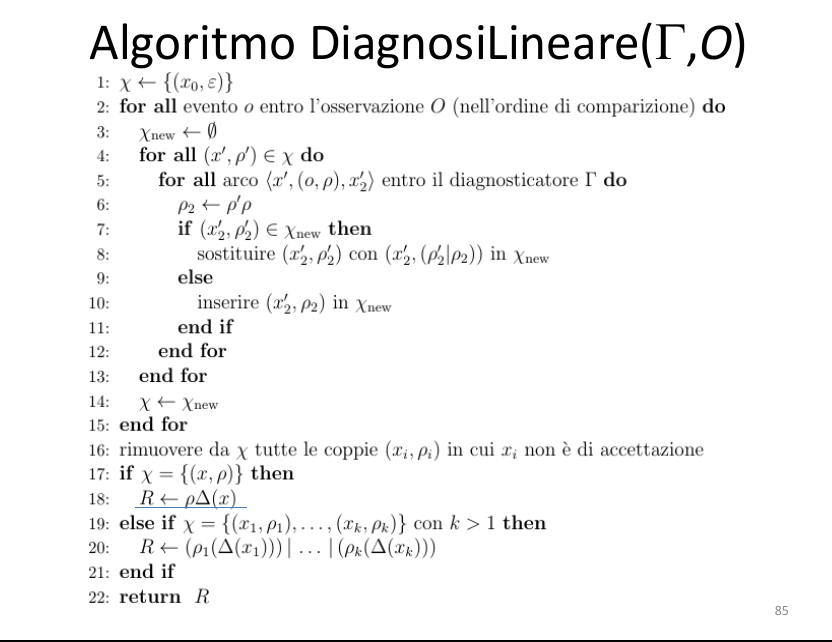
\includegraphics[width=\textwidth]{immagini/diagnosilineare.png}

La funzione responsabile è La funzione responsabile è \textbf{linear\_diagnostic}. I passi per produrre la diagnosi lineare sono i seguenti:. I passi per produrre la diagnosi lineare sono i seguenti:
\begin{enumerate}
    \item produrre la diagnosi lineare: 
    Viene generato un insieme di valori, il cui primo valore è dato dallo stato iniziale del diagnosticatore e da un’etichetta nulla
    \item Successivamente, per ogni etichetta dell’osservazione lineare si recuperano tutti i possibili stati raggiungibili secondo l’etichetta data partendo dal tutti gli stati già raggiunti
    \item Salvati i riferimenti a tutti i passaggi eseguiti (stato-etichetta transizione), si esegue l’algoritmo con una nuova etichetta e i nuovi stati raggiunti nel passaggio precedente, concatenando le etichette delle transizioni su cui si transita
    \item Terminato questo calcolo, si avrà un insieme di stati “attraversati” con varie etichette di rilevanza, si mantengono solo gli stati finali (dunque con un delta esistente) di accettazione. Eventualmente si raggruppano.
    \item Si produce in output una lista di diagnosi concatenando l’etichetta di rilevanza con il delta del relativo stato
    \item Infine si concatenano in OR le diagnosi ricavate
\end{enumerate}

\subsection{Funzioni di supporto}
Le funzioni di supporto, sono state:
\begin{enumerate}
    \item Nel programma principale denominato \textbf{project\_function.py}:
    \begin{enumerate}
        \item \textbf{steps} che raggruppa i singoli passaggi, da \textit{generate\_behavior }a \textit{generator\_diagnosticator}
        \item \textbf{benchmark} per il calcolo del benchmark riducendo all'osso i caricamenti e i salvataggi di file e stampe in stdoutput
    \end{enumerate}
    \item Nel programma contenente solo funzioni di supporto denominato \textbf{extrafunction.py}:
    \begin{enumerate}
        \item \textbf{parse\_arguments} che contiene la logica di esecuzione del parser degli argomenti da linea di comando per l'esecuzioni del programmo
        \item \textbf{json\_to\_obj} per leggere la definizione della rete (in formato json) e creare il relativo oggetto python
        \item \textbf{format\_net\_to\_text} per stampare la definizione della rete
        \item \textbf{clear\_label} per concatenare le stringhe delle etichette in maniera corretta
    \end{enumerate}
    
\end{enumerate}